\documentclass[12pt,a4paper]{article}
\usepackage[utf8]{inputenc}
\usepackage{amsmath}
\usepackage{amsfonts}
\usepackage{amssymb}
\usepackage{graphicx}
\usepackage{booktabs}
\usepackage{natbib}
\usepackage{dcolumn}
\usepackage{setspace}
\usepackage{array}
\usepackage{pdflscape} %allows for rotating pages with wide tables
\newcolumntype{P}[1]{>{\raggedright\arraybackslash}p{#1}}
%\usepackage{tabulary}
\usepackage[T1]{fontenc}
\usepackage{lmodern}
\usepackage{multirow}
\usepackage{multicol}
\usepackage{todonotes}

\usepackage{mathptmx} %times font
%\usepackage{tgpagella} %palatino font
\usepackage[protrusion=true,expansion=true]{microtype}
\usepackage[top=1in, bottom=1in, left=1in, right=1in]{geometry}
\usepackage[hidelinks]{hyperref}
\usepackage{color,soul} %highlighting
\usepackage[size=footnotesize]{caption}
\captionsetup[figure]{labelfont=bf}
\captionsetup[table]{labelfont=bf}

%\usepackage{endnotes}
%\usepackage[heads,nolists,tablesfirst]{endfloat} %places tables and figures at the end
%

%%making use of footnotesize in all tables
\usepackage{floatrow}
\DeclareFloatFont{tiny}{\footnotesize}% "scriptsize" is defined by floatrow, "tiny" not
\floatsetup[table]{font=footnotesize}

%putting caption on top
\usepackage{float}
\floatstyle{plaintop}
\restylefloat{table}

\usepackage{epstopdf}

\usepackage{etoc}
\usepackage{rotating} % Rotating table

\title{\textbf{\Large{When Do Citizens Respond Politically to the Local Economy? Evidence from Registry Data on Local Housing Markets}}}


\author{Martin Vinæs Larsen\thanks{Corresponding author. \href{mailto:mvl@ifs.ku.dk}{\texttt{mvl@ifs.ku.dk}}. } \qquad Frederik Hjorth \qquad Peter Thisted  Dinesen \\Department of Political Science \\ University of Copenhagen \and Kim Mannemar  Sønderskov  \\Department of Political Science \\ Aarhus University   }

%,  }  }


	\begin{document}
	
	\maketitle
	
	\begin{abstract} \noindent Recent studies of how economic conditions shape incumbent support have focused on the role of the local economy, but with inconclusive results. We propose that the impact of the local economy is conditional on which aspects of the local economy voters interact with in their everyday lives. We provide evidence for this proposition by focusing on the influence of local housing markets on support for the incumbent government. Linking uniquely detailed and comprehensive data on housing prices from Danish public registries to both precinct-level election returns and a two-wave individual-level panel survey, we find that when individuals interact with the housing market, their support for the incumbent government is more responsive to changes in local housing prices. The study thus provides a framework for understanding when citizens respond politically to local economic conditions.
		
	\end{abstract}
	
	%\begin{keyword}
	%\doublespacing
	%%x \sep y
	%\end{keyword}
	
	%\end{frontmatter}
	
	\newpage
	
	\onehalfspacing
	%\doublespacing
	
	\section{Introduction}
	
	\noindent Retrospective evaluations of the state of the economy are consequential for voters' electoral choices. Scholars of voting behavior tend to view retrospective voting as an effective shorthand for evaluating the performance of incumbent politicians and for punishing and rewarding them accordingly \citep{ashworth2012electoral,healy2013retrospective}. Yet, the specific aspects of the economy on which retrospective voting is based remain debated. 
	
	After long having focused almost exclusively on either the individuals’ economic situation, or that of the nation she inhabits, the economic voting literature has recently turned its attention to the meso level in terms of local economic conditions. This increased attention has not yet resulted in any scholarly consensus about what role these conditions play in shaping support for incumbent politicians. For example, recent work from \cite{warshaw2017economic} and \cite{healy2017presidential} has found that local economic growth as well as the number loan delinquencies in your area shape support for local and national incumbents in the US. At the same time, work by \cite{wright2012unemployment} ``question[s] the conventional wisdom that incumbent parties are rewarded when unemployment is low and punished when it is high’’ (p. 685). These recent findings from the US are symptomatic of the findings from the existing literature, which are, generally speaking, inconclusive.
	
	The increased attention paid to the role of local economic conditions in the economic voting literature parallels a resurgence of the study of effects of local residential contexts more generally in the political behavior literature \cite[e.g.,][]{hopkins2010politicized,enos2016demolition}. Recent studies have found first-hand exposure to different social phenomena at the local level--at the neighborhood level or even more locally--to be the crucial mechanism underpinning local context effects \citep{moore2017defining,dinesen2015ethnic,enos2016demolition,hjorth2017influence}. This highlights the importance of salient local events as a precondition for effects of local contexts on political behavior to emerge. However, the study of local economic conditions has yet to incorporate this development \citep[though see][]{bisgaard2016reconsidering,reeves2012ecologies}.
	
	In this paper, we join insights on the saliency of local experiences from the broader literature on context effects on political behavior to the economic voting literature to provide a framework for understanding when local economic conditions matter for incumbent evaluations. More specifically, we argue that voters use local economic conditions in their evaluations of government performance, when such features of their local areas are more salient to them. The saliency argument provides an explanation for why local economic conditions only sometimes factor into vote choice, and further helps resolve the tension between positive and null findings in the existing literature.
	
	We test the observable implications of our framework by examining the relationship between changes in local housing markets—a highly salient feature of local economies—and incumbent government support in Denmark, using uniquely detailed and comprehensive data on housing prices. We use two complementary empirical approaches. First, we link detailed registry data on local housing prices to election results at the precinct level across four national elections, allowing us to study whether within-district differences in housing prices are related to support for parties in government. Second, to test the hypothesized causal mechanism—that voters use local housing markets to make inferences about government performance, and more so when housing market is more salient to them—we zoom in on individual voters' local contexts. Specifically, we link a two-period panel survey to very precise measures of how individuals' neighborhoods—measured at very low levels of aggregation—were affected by changes in housing prices.
	
	We find the hypothesized positive relationship between local housing prices and support for governing parties at both the precinct-level and in the individual-level data. Specifically, a 50 pct. year-on-year increase in local housing prices, equivalent to the sharpest price increases during the housing boom, is associated with a 3 to 5 percentage points increase in the support for governing parties. We find no evidence that housing prices affect the respondents’ ideological orientation, and no evidence that the effect of housing prices on incumbent support depends on whether you own your own home. Furthermore, we show that the effect of housing prices is more pronounced among individuals who are more likely to be attuned to the state of their local housing market -- where local housing market activity is high, and among individuals who have recently or soon will be relocating. Taken together, these analyses suggest that voters respond to changes in local housing prices (when salient to them) not because it changes their preferences for specific policy interventions or their own economic situation, but because of what the local housing market tells them about incumbents' performance.
	
	\section{When local economic conditions affect incumbent support}
	
	The extant economic voting literature has primarily investigated whether voters are responsive to local economic conditions in one of two ways. One set of studies has examined the extent to which voters draw inferences about national economic conditions from local economic conditions \citep{books1999contextual,reeves2012ecologies,anderson2011local,ansolabehere2014mecro,bisgaard2016reconsidering}, while another strand of studies have examined the extent to which voters base their support for incumbent politicians on such local conditions \citep{hansford2015reevaluating,eisenberg2004economic,kim2003spatial,healy2017presidential, auberger2005influence,wright2012unemployment}. Studies from both strands of the literature yield inconsistent results finding either small or no effects of local economic conditions on a given outcome.   
	
	Our study distinguishes itself from these previous efforts by highlighting that voters might focus on different parts of the local economy at different times. The average citizen learns about economic conditions through exposure to a multitude of signals from different economic realms. Though she may learn about national economic aggregates through media consumption \citep{soroka2015s}, a substantial part of this exposure to economic signals will inevitably come from local informational sources. This may include casual observation of changing supermarket prices, shuttered stores, or job postings. She may also learn about local economic conditions from direct, personal involvement with the local economy through job search or buying or selling a home. Each of these interactions involves exposure to a particular aspect of the local economy.
	
	The notion that citizens learn about national-level conditions through particular aspects of local economic conditions has a long pedigree in studies of public opinion and voter behavior. Lippmann \citeyearpar[][p. 79]{lippmann1946public} observed that ``we see at best only a phase and an aspect’’ of public events. Discussing learning about economic conditions specifically, Popkin \citeyearpar[][p. 24]{popkin1994reasoning} notes that ``[p]olitical information is acquired while making individual economic decisions and navigating daily life: shoppers learn about inflation of retail prices; home buyers find out the trends in mortgage-loan interest rates; owners of stock follow the Dow-Jones averages (...)’’ \cite[see also][p. 5]{fiorina1981retrospective}. However, even while acknowledging this point, scholars have refrained from theorizing when particular aspects affect citizens’ evaluations of incumbents. 
	
	We focus on a particular aspect of the local economy, namely housing, for several reasons. First, housing markets saw a global boom followed by a bust in the period around the great recession with severe economic implications for well-being of both individual households and the overall state of the economy. Second, governments influenced the severity of the market crash to a considerable extent through housing and monetary policy, which in turn makes it likely that voters attribute responsibility to them. Third, housing markets are not a monolithic national phenomenon, but vary substantially across geographical contexts, thereby providing voters with highly visible local information by which to assess incumbents. 
	
	As our first hypothesis, we expect citizens to treat rely on information from local housing markets when assessing the performance of incumbents: 
	
	\newcommand{\hone}{the local economic conditions hypothesis}
	
	\begin{quote}
		\textit{H1 (Local economic conditions hypothesis): When local housing prices rise, individuals are more likely to support the incumbent government.}
	\end{quote}
	
	We argue that in the process of a citizen interacting with a particular aspect of the local economy, that aspect becomes cognitively salient. When she evaluates the incumbent government’s economic performance in the context of vote choice, aspects with which she has interacted more recently are more likely to factor in as ``top-of-mind’’ considerations \citep{zaller1992nature}. The concept of priming in the political psychology literature provides an instructive parallel. Just as media emphasis on particular political issues in the context of a campaign can cause those issues to carry more weight in a citizen’s evaluation of the incumbent, interaction with a particular aspect of the local economy can cause that aspect to carry more weight in her assessment of the state of the local economy in general. In that sense, our argument applies the logic of priming to citizens’ interactions with and evaluations of local economic conditions. In doing so, we follow in the footsteps of earlier work examining how national-level events can prime local conditions \citep[e.g.,] []{hopkins2010politicized,legewie2013terrorist}. 
	
	This leads to out second hypothesis, namely that the association posited in H1 is stronger where local economic activity primes housing market information:
	
	\newcommand{\htwo}{the contextual priming hypothesis}
	
	\begin{quote}
		\textit{H2 (Contextual priming hypothesis): The association between changes in local housing prices and support for the incumbent government is stronger when individuals are more exposed to local housing market activity.}
	\end{quote}
	
	This conditional theory of how local economic conditions matter for voters might help explain why previous studies have found inconsistent results. If the impact of local economic conditions depends on which aspects of the local economy citizens interact with, then we should expect the effect of local economic conditions to be moderated by what kind of local economic conditions the study focuses on and by the relation that the electorate has to this part of the economy.
	
	In addition to the literature on the impact of local economic conditions referenced above, our study ties into several neighboring literatures. First, as already highlighted, our study builds on and adds to the growing literature on `context effects' exploring the various ways in which political behavior and conditions are shaped by local contexts \citep[e.g.,][]{hopkins2010politicized,enos2016demolition}. Second, our study also ties in with a recently emerged strand of research in political economy highlighting the influence of home ownership -- in itself or as part of a portfolio of economic assets -- on redistribution and social policy preference as well as voting \citep{ansell2014political,nadeau2010patrimonial,stubager2013reaching}.
	
	\section{Empirical setting}
	
	We study the effect of changes in local housing prices on support for the incumbent government in Denmark in the years surrounding the onset of the Great Recession. The precinct-level data (cf. Section \ref{precinctlevel}) covers the election years of 2005, 2007, 2011, and 2015, whereas the individual-level data (cf. Section \ref{individuallevel}) covers responses from a two-wave panel survey collected in 2002, 2004, 2008, and 2011. Denmark is a particularly useful setting for studying the hypothesized during this period of time due to large temporal variations in housing prices. The boom and bust of the Danish real-estate market before and during the great recession were large, even by international standards. Figure \ref{hpd} shows the trajectory of Denmark's housing bubble compared with other prominent international cases.
	
	\begin{figure}[htbp!]
		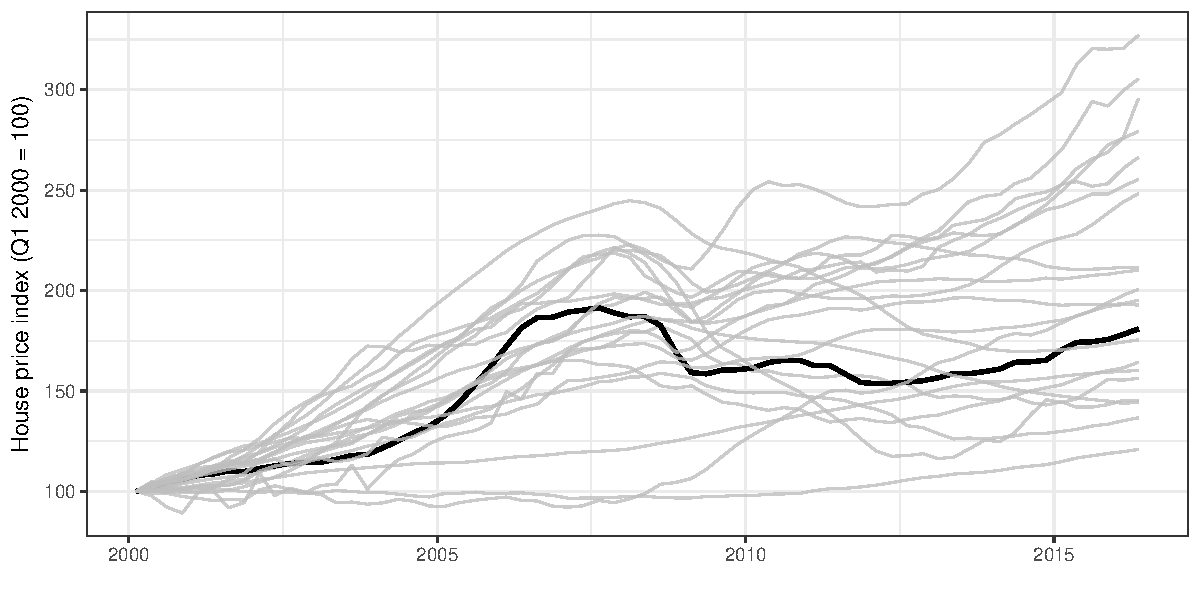
\includegraphics[width=0.9\textwidth]{../figures/timeplot}
		\centering
		\caption{Trends in real housing prices in Denmark (black line), Spain, the UK, and the US (dark gray lines) and selected other countries (light gray lines), 2000-2016 (2000 level = 100). Based on the International House Price Database maintained by the Dallas Fed. The authors acknowledge use of the dataset described in Mack and Martinez-Garcia (2011).}\label{hpd}
	\end{figure}
	
	As shown in Figure \ref{hpd}, although many economies experienced large increases in real housing prices, Denmark's housing bubble was exceptionally volatile, characterized by a late, rapid increase quickly succeeded by an equally rapid crash. The bulk of Denmark's housing boom and bust occurred in just four years, from 2005 to 2009. In contrast, the housing bubble in the United States (highlighted in Figure \ref{hpd}), although far bigger in absolute terms, was relatively protracted in comparison. Consequently, local housing markets in Denmark saw year-to-year changes in housing prices that were, even by the standards of a globally economically volatile period, unusually large. This provides us with ample variation in the independent variable of interest.
	
	The policies exacerbating the housing bubble were implemented by the conservative government holding office from 2001 to 2011. This renders support for the incumbent government observationally indistinguishable from voters becoming more ideologically conservative, a plausible consequence of increases in housing wealth \citep{ansell2014political}, in the individual-level data that only cover this period. To distinguish between such an ideological effect of increases in housing prices and a typical non-ideological economic voting effect by investigating whether the size of our effect estimates depend on the ideology of the incumbent government. 
	
	%In Section \ref{inference}, we exploit the change in incumbency in 2011-2015 to show that housing price changes affect support for the incumbent government per se, not merely support for a conservative government.
	
	%Turning to the political context, the government in the entire period we investigate (2005-2015) consisted of two different parties. From 2001 to 2011 the Liberal party was in government along with the Conservative party, and from 2011 till 2015 the Social Democratic party and the Liberal party was in power.\footnote{An additional party, the Socialist party, was in government from 2011 to 2013, however, since this party left government before the election, it is excluded when looking at electoral support for the governing party. To get data on electoral support at the previous election, we also use some data from the 2001 election in which the Social Democratic party and the Liberal party was in power.} This change in party incumbency is useful, since it allows us to distinguish effects on incumbent government support from effects on macropartisanship.
	
	%Housing markets saw a boom followed by a bust in the period around the great recession. This had severe economic implications for wellbeing of both individual households’ and the overall state of the economy \citep{dam2011housing,ansell2014political}. Pairing the economic importance of the housing market with the fact that government regulations (or lack thereof) to a considerable extent influenced the severity of the market crash makes housing markets a particularly useful mean for voters to evaluate the incumbent government by. Furthermore, housing markets are not a monolithic national phenomenon, but vary substantially across geographical contexts, thereby providing voters with relevant local information by which to assess incumbents.
	
	%The second reason we focus on Denmark, is that it is possible to obtain precise and comprehensive data on housing price changes, voting returns, and socio-economic controls at a very small geographic level. Existing approaches typically examine housing price returns at high levels of aggregation corresponding to either counties or entire states. In contrast, we observe housing price changes at the zip code level and voting returns and socio-economic controls at the precinct (i.e., polling place) level. This allows for much more precise measurements of the variables of interest and accordingly less attenuation of observed associations. We elaborate on the specifics of the data in the next section.
	
	\section{Research design and data}\label{resdesign}
	
	Methodologically, we advance the study of the role of local housing markets in economic voting by exploiting comprehensive and highly granular data on housing market transactions available in Danish public registries. Specifically, we link highly detailed register data on local housing prices to both precinct-level panel data on national election outcomes as well as individual-level survey data. These data ameliorate three methodological challenges confronting previous studies of the role of local economic context as well as the broader class of studies scrutinizing local influences on political attitudes and behavior.
	
	First,  by utilizing precise and highly local measures of housing prices drawn from public registries we address the common problem of confounding local contexts with local media markets – an entirely different mechanism. Distinguishing between the two influences is rarely possible due to data constraints, specifically focusing on local economic conditions in more aggregated geographical contexts, where local context and local media markets overlap \citep[][]{bisgaard2016reconsidering}.  
	
	Second, and related to the previous point, measures of local economic conditions are often sample-based, which makes the estimation of conditions at lower geographical levels imprecise and therefore causing attenuation bias (i.e. a downward bias) in the estimated relationship \citep[][]{healy2017presidential}. We avoid such problems through the use of data from the full population, and can therefore measure local housing prices with very high precision.
	
	Third, most previous studies have relied on cross-sectional data \citep[][]{bisgaard2016reconsidering, reeves2012ecologies, ansolabehere2014mecro, books1999contextual}. While such data are often the best at hand, they come with the risk of confounding a relationship between local housing prices and support for incumbents by structural economic differences (e.g. differences in industry composition) between local contexts. This is perhaps best exemplified by the strong urban-rural gradient in local economic conditions, which would likely confound any observed cross-sectional relationship with support for the sitting government. By using panel data, we can rule out confounding by such time-invariant structural differences between local contexts by using only within-precinct/within-individual variation in local housing prices by means of fixed effects.
	
	Some previous studies address some of the noted methodological challenges, but our study is, to the best of our knowledge, the first to address all of these at once. In the remainder of this section, we present in more detail the two data sources we use two test our hypotheses; a precinct-level and an individual-level data set.
	
	\subsection{Precinct-level data}\label{precinctlevel}
	We begin our analysis of the relationship between the state of local housing markets and incumbent support by looking at precinct-level election returns in Danish Parliamentary elections between 2005 and 2015. More specifically, we match electoral support for parties in government in these precincts with change in the price of all house sales in and around the precincts, examining the extent to which local housing prices and local electoral support for government parties go hand in hand.
	
	
	The dependent variable in this analysis is \textit{percent of votes cast for government parties} in voting precincts. Each voting precinct corresponds to a single polling place, which is the smallest unit at which voting returns can be observed in Danish elections. We measure this for all precincts in four elections:  2005, 2007, 2011 and 2015. There are roughly 1,400 precincts, each precinct consisting of about 3,000 eligible voters on average and covering an average area of 30 square kilometers. A number of precincts are redistricted between each election. This is problematic, as we want to use the precincts as part of a panel data set. One way to deal with this is to drop precincts as their geographical boundaries get altered. As a consequence, roughly 15 pct. of the data on the dependent variable would be dropped. We therefore opted for an alternative solution, namely to fix the precincts geographical boundaries at one reference election (i.e. 2015), and then recalculate vote returns in any changed precincts, so they match up with precincts in the reference election. We believe this strategy, allowing us to use the full sample precincts, is preferable as the changes in geographical boundaries from election to election are generally minor with only a few major changes\footnote{For details of how returns from the redistricted precincts are calculated, see Søren Risbjerg Thomsen's research note at \texttt{\href{http://bit.ly/205OlPi}{bit.ly/205OlPi}}.  We use 2015 as the reference election.}
	
	The key independent variable is \textit{change in local housing prices}. We obtain housing price data from The Danish Mortgage Banks' Federation (\textit{Realkreditforeningen}), which publishes quarterly data on the average price per square meter of all sales at the zip code level, aggregated from registry data on individual sales.\footnote{Available at \texttt{\href{http://statistik.realkreditforeningen.dk/}{statistik.realkreditforeningen.dk}}.} For each election, we calculate change in housing prices as the percentage change in the price of houses sold in the quarter of the election compared to the same quarter one year before. We merge observations of house prices and incumbent support by assigning every polling station to the year-on-year price change in its zip code. We provide additional details on this assignment procedure in appendix \ref{app_linking}.
	
	The dependent variable is a measure of changes in prices rather than price levels. This choice is in part motivated by the well-documented general tendency of human perceptions to be more responsive to changes in conditions than to absolute levels \citep{kahneman1979prospect}. It is also in keeping with the extant economic voting literature which, to the extent that it has looked at prices, has had a similar focus on changes (i.e., inflation, e.g. \citealp{kramer1971short}). At the local level, changes in housing prices will translate into shorter or longer turnaround times, as sellers and buyers try to adjust to the new prices, leaving visible traces of these changes in the voters’ immediate context. These visible traces may take the form of ``for sale’’ signs in front yards and windows, or the speed at which old neighbors are exchanged for new ones.
	
	In the statistical models, we control for the unemployment rate and median income at the zip-code level in order to isolate local housing markets from other features of the local economy. Like the independent variable, these are population-based measures calculated from public registries provided by Statistics Denmark.
	% To account for potential confounding from differences between urban and rural housing markets, we also control for the population density ($log(\frac{inhabitants}{km^2})$) of the municipality in which the precinct is located.
	
	\subsection{Individual-level data}\label{individuallevel}
	%In the preceding analysis, we have shown the hypothesized relationship between local housing prices and support for incumbents at the precinct level. While this is quite strong evidence in its own right, replicating this finding using the individual-level data would strengthen its credibility. 
	
	Although our precinct-level data is comprehensive, our hypotheses are at the individual level, and testing individual-level theories with aggregate-level data is fraught with problems of ecological inference. Hence, we include data from a representative sample of Danish citizens in a two-wave panel survey collected between 2002 and 2011. We link the survey respondents to the prices of housing sold in their residential context using the national Danish registers. The registers contain very detailed information about all individuals legally residing in Denmark, including the exact geographical location of their residence, the price of any real estate they sell, and a range of other socio-demographic characteristics \citep{thygesen2011introduction}. This makes it possible to calculate the distance between the individuals in the survey and all other individuals in Denmark and, in turn, the distance to any individuals who are selling their home.
	
	In addition to observing voting behavior at a more theoretically appropriate level, the individual-level data employed also offer a number of features which allow us to probe the hypothesized relationship further. The flexibility and detail of the Danish registers makes it possible to look at multiple levels of aggregation rather than just levels of aggregation generated for administrative use such as zip codes. This makes it possible to reduce concerns related to the modifiable area unit problem (MAUP)—a thorny issue within contextual research in general—in that we can rule out that the findings are tied to a particular way of geographically aggregating housing prices. Furthermore, we can link housing prices to individual-level variables such as home ownership, which allow for evaluating plausible alternative explanations. 
	
	To get at support for governing parties at the individual level we utilize a two-wave panel survey, constructed by re-interviewing respondents who had participated in the Danish Version of the European Social Survey (ESS); a nationally representative high-quality survey conducted bi-annually in most European countries. The first round of the survey was conducted at three different points in time (round 1, 2 and 4 of the ESS): 2002/3, 2004/5 and 2008/9. In the second round, the full sample of ESS round 1 and 4, and 40 pct. of ESS round 2 (randomly selected), were invited for a re-interview in the winter of 2011-12. In total, 1,745 people -– equivalent to a retention rate of 47 pct. -– were interviewed in both rounds.
	
	The respondents were randomly sampled from the public registry, and therefore the civil registration numbers were retained by the data collection agency. This made it possible to identify the respondents for a second interview and to link the respondents to the national registers. From the survey, we use the following question: ``What party did you vote for at the last parliamentary election?’’. Respondents were presented with all the parties which ran in the previous election. For the analyses we create a dummy variable indicating whether the respondent voted for a party in government at the time of the election as the dependent variable.
	
	
	Our independent variable is again year-over-year changes in housing prices in the residential context of the respondent. We measure the change by comparing the price of housing sold in the quarter prior to the data collection and the price of housing sold in the same quarter a year earlier. Unlike for the precinct-level data, we do not have data on prices per square meter. This makes the individual-level housing price change variable more sensitive to random variation in the types of housing put up for sale in the two time periods we compare. As such, year-to-year changes in prices may partly that larger houses were put up for sale in a given year. To take this as well as other structural differences in the type of housing put up for sale into account, we divide the sales price of each unit of housing by its public valuation, before calculating the year-over-year change.\footnote{The Danish government makes a conservative estimate of the price of all housing in Denmark every two years which is used to calculate property taxes. The public evaluation was constant across the time periods we use to estimate housing price changes.}
	
	We estimate the changes in housing prices within each survey respondent's residential context, measuring this context in three different ways. First, and similar to what we did for the precinct-level data, we use the respondents’ zip-code, comparing housing sold within the same zip code a year apart. Second, we look at the prices of the 20 or 40 units of housing sold closest to the respondents own home, comparing the prices of housing sold in the immediate proximity of the respondent to that of housing sold one year earlier. Third, we look at the price of housing sold within a fixed radius of 1000 or 1500 meters of the respondent. These latter ways of defining the respondents’ residential contexts have the benefit of being centered on the respondent, alleviating the problem that the context of a respondent living far from the centroid of one zip-code might be better represented by an adjoining zip-code. Note also that these latter two types of residential context differ in important ways: whereas the first method takes number of sales as fixed, but varies the geographical dispersion of these sales, the second method holds geographical dispersion fixed, but varies the number of sales. To assess the robustness of our results, we probe the relationship between local housing prices and incumbent support using all of the above measures.\footnote{See Appendix \ref{app_housingselect} for details of how we arrive at the housing price estimates.}
	
	Lastly, for evaluating \htwo, we develop a measure of individual-level exposure to the local housing market. We construct a variable from public registries whether the respondent moved within six months before or after being surveyed. The variable takes the value of one if respondents move within this period of time and zero otherwise. This variable can be viewed as a proxy for whether respondents are interacting with the housing market and thus whether they were exposed information about the trajectory of housing prices.
	
	We include a number of additional variables in the analysis for statistical control, interaction analyses and placebo tests, which we present as we introduce them in the analysis. 
	
	
	
	\section{Precinct-level evidence}
	Table 1 evaluates the proposition that local housing prices help the incumbent government through a set of linear regression models. The table presents the estimated effect of year-over-year changes in housing prices on electoral support for the parties in government. All models are estimated using robust standard errors clustered at the precinct-level. The first model is a simple linear regression between electoral support and changes in housing prices. The second includes year fixed effects, holding trends in incumbent support and rates of housing price changes constant, and the third includes precinct fixed effects as well. In effect, model 3 is a difference-in-difference model, that evaluates whether electoral support increases or decreases more in precincts where housing prices increase more.  In the fourth model, we include the unemployment rate and the median income as covariates, controlling for overall  trends in the precincts’ economic situation. 
	
	\begin{table}[htbp]\centering
\def\sym#1{\ifmmode^{#1}\else\(^{#1}\)\fi}
\caption{Estimated effects of house prices on electoral support for governing parties.} \label{predv}
\begin{tabular}{l*{4}{c}}
\hline\hline
                    &\multicolumn{1}{c}{(1)}        &\multicolumn{1}{c}{(2)}        &\multicolumn{1}{c}{(3)}        &\multicolumn{1}{c}{(4)}        \\
\hline
$\Delta$ housing price&       0.104\sym{**}&       0.048\sym{**}&       0.053\sym{**}&       0.030\sym{**}\\
                    &     (0.008)        &     (0.007)        &     (0.008)        &     (0.007)        \\
[1em]
Unemployment rate   &                    &                    &                    &      -1.898\sym{**}\\
                    &                    &                    &                    &     (0.221)        \\
[1em]
Log(Median income)  &                    &                    &                    &      -0.891\sym{**}\\
                    &                    &                    &                    &     (0.064)        \\
[1em]
\hline Year FE      &                    &$\checkmark$        &$\checkmark$        &$\checkmark$        \\
[1em]
Precinct FE         &                    &                    &$\checkmark$        &$\checkmark$        \\
\hline
Observations        &        4193        &        4193        &        4193        &        4173        \\
RMSE                &       8.403        &       6.748        &       5.713        &       5.321        \\
\hline\hline
\multicolumn{5}{l}{\footnotesize Standard errors in parentheses}\\
\multicolumn{5}{l}{\footnotesize \sym{*} \(p<0.05\), \sym{**} \(p<0.01\)}\\
\end{tabular}
\end{table}

	
	Table \ref{predv} shows that there is a statistically significant and positive coefficient attached to changes in housing prices, indicating that a larger fraction of the electorate casts their vote for governing parties in precincts where housing prices are increasing. In the most demanding specification the coefficient is 0.03, which implies that when the price of housing sold in a precinct's zip-code doubles from one year to the next, electoral support for governing parties in this precinct increases by roughly 3 percentage points.
	
	Unsurprisingly, the effect is larger in the less restrictive models. The effect size drops from 0.1 to 0.05 when introducing the economic controls, and drops additionally to 0.03 when introducing the time and precinct fixed effects. This highlights the strength of using a difference-in-difference approach and controlling for detailed information about other aspects of the local economy, as this evidently picks up important sources of confounding.
	
	Yet, a potential threat to our results is that that the effect of local housing markets on support for incumbents is a reflection of some secular trend predating changes in housing prices -- i.e., that governing parties were already becoming more/less popular in places where housing prices eventually increase/decrease. To address this concern about violation of the parallel trends assumption, we estimate the same type of models as in Table \ref{predv} using support for the governing party at the \textit{previous election} as the dependent variable (i.e. the lagged dependent variable). If we observe a significant relationship between prior support for incumbents an subsequent rises in housing prices, this would indicate that the parallel trends assumption is violated. We plot the estimated effects of housing prices on the lagged dependent variable as well as on the actual dependent variable in Figure \ref{placebo}. The figure shows a significant effect of housing prices on the lagged dependent variable in the less restrictive models. However, in the final and most restrictive model, the estimated effect of housing prices on lagged incumbent support is 0.005 -- less than a sixth of the estimate on subsequent support; cf. in the corresponding model in Table \ref{predv} -- and statistically insignificant. This indicates that pre-treatment trends in treated and non-treated units are indeed parallel.
	
	%Finding that prior trends in the dependent variable are uncorrelated with the independent variable, is important as this indicates that a key assumption (i.e. the parallel trends assumption) underlying the difference-in-difference model holds up. 
	
	\begin{figure}[htbp!]
		\includegraphics[width=0.9\textwidth]{../figures/lagdv.eps}
		\centering
		\caption{Effects of Housing Prices on support for governing party at the present election (t) and the last election (t-1) with 90  and 95 pct. Confidence Intervals}\label{placebo}
	\end{figure}
	
	
	
	
	
	We proceed to evaluate \htwo, testing whether the relationship between changes in local housing prices and incumbent support is moderated by local housing market activity. Table \ref{table:econactivity} reports a set of models similar to those presented in Table \ref{predv}, but with changes in housing prices interacted with the (logged) number of trades in the preceding quarter. We observe a statistically significant interaction between local housing prices and market activity: the association between housing prices and incumbent support is stronger in areas with higher levels of housing market activity. 
	
	
	\begin{table}[htbp]\centering
\def\sym#1{\ifmmode^{#1}\else\(^{#1}\)\fi}
\caption{Estimated effects of housing price across number of trades.} \ref{table:econactivity}} \label{prelagiv}
\begin{tabular}{l*{4}{c}}
\hline\hline
                    &\multicolumn{1}{c}{(1)}        &\multicolumn{1}{c}{(2)}        &\multicolumn{1}{c}{(3)}        &\multicolumn{1}{c}{(4)}        \\
\hline
$\Delta$ housing price&      -0.039        &      -0.102\sym{**}&      -0.077\sym{**}&      -0.079\sym{**}\\
                    &     (0.027)        &     (0.021)        &     (0.023)        &     (0.023)        \\
[1em]
$\Delta$ housing price $\times$ logntrades&       0.049\sym{**}&       0.050\sym{**}&       0.038\sym{**}&       0.033\sym{**}\\
                    &     (0.008)        &     (0.007)        &     (0.007)        &     (0.007)        \\
[1em]
Unemployment rate   &                    &                    &                    &      -1.656\sym{**}\\
                    &                    &                    &                    &     (0.217)        \\
[1em]
Log(Median income)  &                    &                    &                    &      -0.856\sym{**}\\
                    &                    &                    &                    &     (0.063)        \\
[1em]
\hline Precinct FE  &                    &                    &$\checkmark$        &$\checkmark$        \\
[1em]
Year FE             &                    &$\checkmark$        &$\checkmark$        &$\checkmark$        \\
\hline
Observations        &        4195        &        4195        &        4195        &        4175        \\
RMSE                &       8.501        &       6.736        &       5.637        &       5.288        \\
\hline\hline
\multicolumn{5}{l}{\footnotesize Standard errors in parentheses}\\
\multicolumn{5}{l}{\footnotesize \sym{*} \(p<0.05\), \sym{**} \(p<0.01\)}\\
\end{tabular}
\end{table}

	
	\begin{figure}[htbp!]
		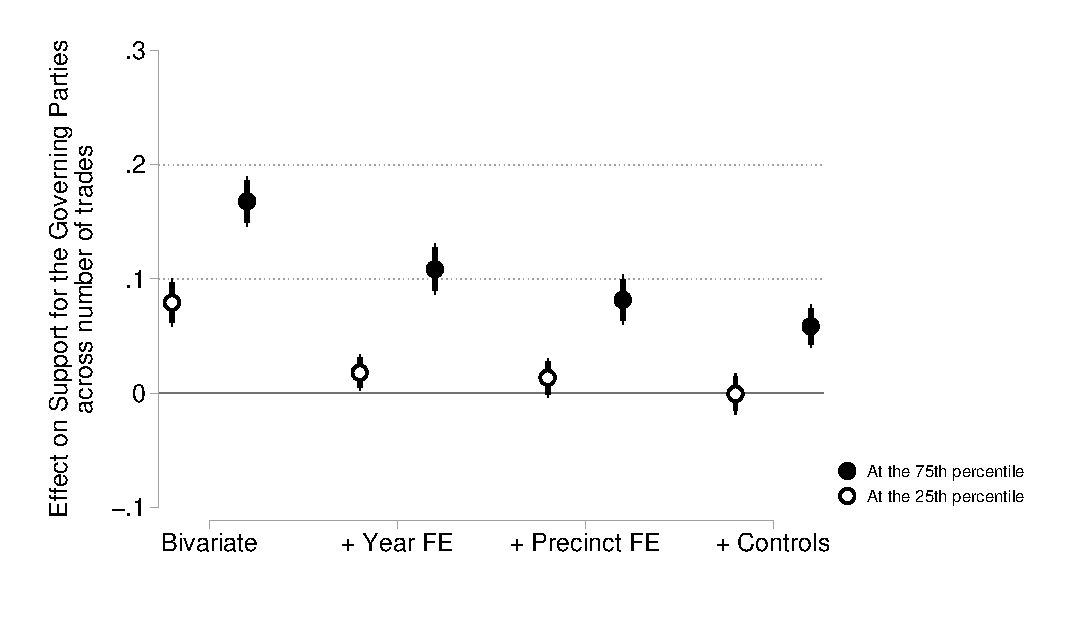
\includegraphics[width=0.9\textwidth]{../figures/localactivity.eps}
		\centering
		\caption{Marginal effects of housing prices across levels of economic activity with 90  and 95 pct. Confidence Intervals.  Marginal effects derived based on table \ref{table:econactivity} at the 25th and 75th percentile.}\label{localactivity}
	\end{figure}
	
	Since interaction models can be difficult to interpret based on reported coefficients alone, we visualize the result in Figure \ref{localactivity}. For each model specification, the figure shows the predicted effect of local housing prices on incumbent support for zip code economic activity corresponding to  the 25th and 75th percentile. The most notable result is that for the most restrictive model, there is essentially no effect at the bottom 25th percentile, while the effect is about twice the size of the average effect  (i.e., 0.06) at the 75th percentile. We thus find clear support for \htwo. In localities where the local housing market is more active, and thus where voters plausibly pay more attention to local housing markets, these markets feature more prominently in the evaluation of incumbents. One potential concern could be that housing prices and market activity measure the same underlying phenomenon. As we discuss below and in Appendix \ref{app_interaction}, the two are very weakly correlated, leaving ample room for the two to vary independently.
	
	\subsection{Auxiliary analyses and robustness checks}
	Table \ref{robustness} presents a series of robustness checks of the results presented above. For these analyses, we only report the estimated average effect of housing prices and the interaction between (logged) number of trades and housing prices. The full models are reported in Appendix \ref{app_robustpred} of the supplementary materials.
	
	\begin{table}[htbp]\centering
	\def\sym#1{\ifmmode^{#1}\else\(^{#1}\)\fi}
	\caption{Assesing the Robustness of the Precinct-level Evidence} \label{robustness}
	\begin{tabular}{l*{4}{c}}
		\hline\hline
		&\multicolumn{1}{c}{(1)}        &\multicolumn{1}{c}{(2)}        &\multicolumn{1}{c}{(3)}        &\multicolumn{1}{c}{(4)}        \\
\hline
$\Delta$ housing price (2 years)&       0.129\sym{**}&       0.037\sym{**}&       0.022\sym{**}&       0.020\sym{**}\\
&     (0.007)        &     (0.007)        &     (0.007)        &     (0.007)        \\
[1em]
$\Delta$ housing price (FD controls)&       0.104\sym{**}&       0.073\sym{**}&       0.086\sym{**}&       0.058\sym{**}\\
&     (0.008)        &     (0.008)        &     (0.009)        &     (0.008)        \\
[1em]
$\Delta$ housing price (FD DV)&       0.037\sym{**}&       0.034\sym{**}&       0.052\sym{**}&       0.019\sym{**}\\
&     (0.004)        &     (0.004)        &     (0.005)        &     (0.004)        \\
[1em]
$\Delta$ housing price (negative)&      -0.081\sym{***}&      -0.072\sym{***}&      -0.057\sym{**} &      -0.030         \\
&     (0.022)         &     (0.017)         &     (0.019)         &     (0.019)         \\
[1em]
$\Delta$ housing price (positive)&       0.116\sym{***}&       0.045\sym{***}&       0.031\sym{**} &       0.029\sym{*}  \\
&     (0.012)         &     (0.011)         &     (0.011)         &     (0.011)         \\
[1em]
\hline Economic controls  &                    & $\checkmark$                    &$\checkmark$        &$\checkmark$        \\
[1em]
Precinct FE  &                    &                    &$\checkmark$        &$\checkmark$        \\
[1em]
Year FE             &                    &                    &                    &$\checkmark$        \\
\hline\hline
\multicolumn{5}{l}{\footnotesize Standard errors in parentheses}\\
\multicolumn{5}{l}{\footnotesize \sym{*} \(p<0.05\), \sym{**} \(p<0.01\)}\\
\end{tabular}
\end{table}
	
	We begin by looking at whether the chosen time period, i.e. year-over-year changes, affects the results. To do so, we reestimate the most restrictive model from tables \ref{predv}--\ref{econactivity} using the change in housing prices over two years rather than just one. The results, reported in the first row in Table 2, are fairly similar using this measure of more long run changes in housing prices, although the estimated effects tend to be smaller than what reported above. This squares with previous work showing that voters are, by and large, myopic when it comes to relating economic indicators to incumbent support \citep{healy2009myopic,healy2014substituting}.
	
	As mentioned above, we use changes in housing prices rather than levels. However, in our models we control for the level of income and the level of unemployment. As a consequence,  we may fail to capture something important about how the economic status of the precinct is changing, which could in turn confound the effect of changes in housing prices. To examine whether this is the case, we re-estimate the different models using first-differenced (FD) controls. As can be seen in the second row of Table \ref{robustness}, this does not alter the main conclusion. In fact, the estimated effects of local housing prices doubles in size in this specification. We also estimate a set of complete change models using an FD dependent variable. The estimates from these models are reported in the third row of Table \ref{robustness}. While somewhat smaller, the effect of housing prices remains statistically significant in the completely differenced model.
	
	To test for nonlinearities in the observed relationship, we split the housing price variable in two, creating one variable measuring the size of positive changes with negative changes set to zero, and another one measuring the size of negative changes with positive changes set to zero. This makes it possible to study the effect of increases and decreases in housing prices separately. We report the result of these analyses in the last two rows of Table \ref{robustness}. Interestingly, we find no evidence of negativity bias: the effect of negative changes and positive changes are both roughly 0.03. This symmetry is important because it shows that voters not only reward governing politicians when housing prices are on the rise, but also punish them when they fall. Moreover, the effect of both positive and negative changes are both conditioned by the number of trades.  This contrasts with earlier studies finding that voters respond more strongly to negative economic changes \citep[e.g.][]{bloom1975voter,headrick1991attention,soroka2014negativity}. 
	
	
	Another concern relates to whether the effect is only present for right-wing incumbents. As housing prices in an area increases, the wealth of the voters living in this area also increases on average, which might lead to increased support for right-wing politicians \cite{ansell2014political}. This problem is especially acute in our data, as the government parties in power from 2001 to 2011 were right-wing. To address this concern, we estimate models predicting support for the left-wing government coalition (Social Democratic party and Social Liberal Party) and the right-wing government coalition (Liberal Party and Conservative Party) using housing prices, precinct and year fixed effects, as well as the local economic controls. We then interact the housing prices measure with a binary indicator for whether the parties are in office.\footnote{We estimated this model on a dataset which included all precinct-years twice: once with the left-wing coalition support and once with right-wing coalition support. The housing price effect is conditioned on a two-way interaction between government coalition (i.e., whether we are predicting support for left-wing or right-wing government coalition) and whether this coalition is in office. See Appendix \ref{app_partyspec} in the supplementary materials for the full model.} Figure \ref{partyspecific} presents the key estimates from this model, showing that increasing housing prices have a positive effect on electoral support for both right-wing and left-wing parties when these parties are in office. Our result can thus not be explained solely by increased housing wealth causing a conservative shift in the electorate. This is important because it implies that the relationship between changes in local housing prices and support for incumbent governments is independent of the partisan composition of the government.
	
	\begin{figure}
		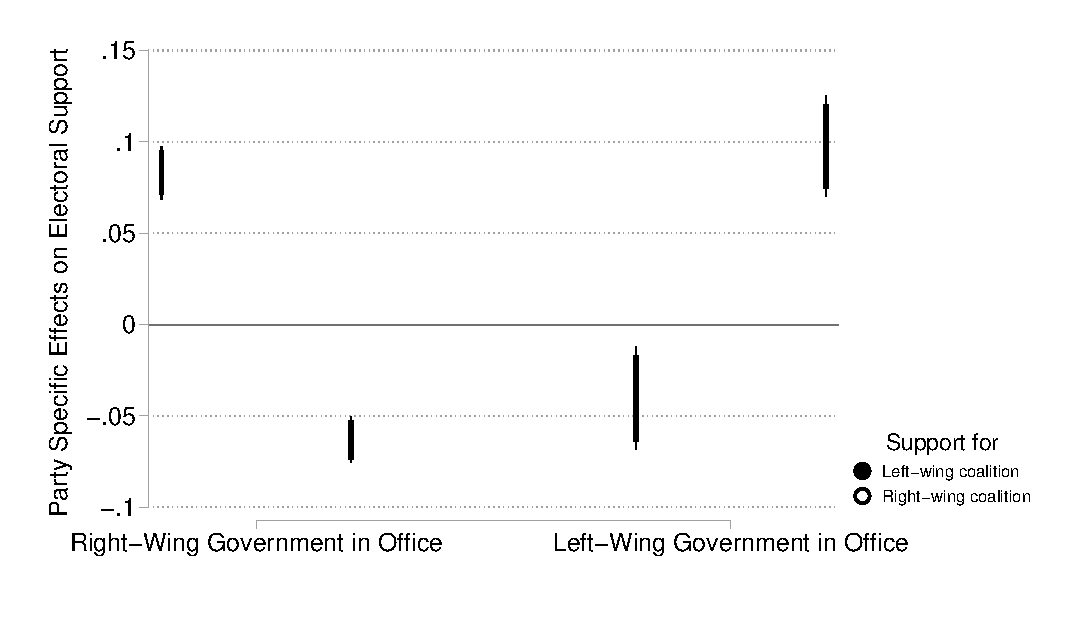
\includegraphics[width=1\textwidth]{../figures/partyspecific.eps}
		\caption{The marginal effect of housing prices on electoral support for either the left-wing or the rigt-wing government coalition conditional on which coalition is in office. See Appendix \ref{app_partyspec} of the supplementary materials for the model underlying this figure.}
		\label {partyspecific}
	\end{figure}
	
	Finally, one might have some specific concerns with respect to the interaction model. One concern is that number of trades measures the same underlying feature of the local housing market (i.e. rising activity is reflected in rising prices), making any interaction analysis nonsensical. However, the two variables are very weakly correlated ($r=0.1$). Further, one might suspect that the interaction term is non-linear. Using the binning estimator developed  by Hainmueller, Mummolo and Xu (2017), we find some evidence of this, as the effect of housing prices only seems to materialize in the upper tercile of the moderator. However, such a non-linearity seems perfectly consistent with \htwo  (see Appendix \ref{app_interaction} for a more detailed analysis). 
	
	In sum, we find clear evidence for both \hone and \htwo in the precinct-level data. We now proceed to testing the hypotheses using the individual-level data.
	
	\section{Individual-level evidence}
	
	In Table \ref{inddv} we report results from a set of linear probability models, estimating the probability of voting for a party in government as a function of changes in local housing prices. We choose to estimate linear probability models in the interest of simplicity, but we show in Appendix \ref{app_robustind} that the results are virtually similar when estimated using logistic regression. We include individual (respondent) fixed effects, and fixed effect for which of the four different survey rounds the respondent initially participated in (ESS rounds one, two or four). All models include controls for the average income and unemployment rate in the respondent's context, as well as indicators of the respondent's own income and whether someone in the household is unemployed. Like in the precinct-level analyses, we include these controls to differentiate the effect of local housing markets from trends in the overall economic circumstances. However, unlike for the precinct-level data we can now control for trends in both the respondent’s personal economy and for the economy of the larger context. In effect, we end up with a similar identification strategy as for the precinct-level data: a difference-in-difference model that controls for trends in the economic situation. All models include robust standard errors clustered at the individual-level.
	
	All models include the same set of variables, but differ in how the contextual variables are defined. In column one we present a model where housing price change is calculated based on the 20 sales closest to each respondent, and where the other contextual variables -- average income and unemployment rate -- are measured within a 500 meter radius of each respondent. In column two we use the 40 closest sales, but leaves the remaining variables measured as in column one. In columns three and four we define all contextual variables (house prices, unemployment rate and average income) as based on 1000 and 1500 meter radii around the respondent. Finally, in column five, we examine sales at the level of zip codes, but the other contextual variables are calculated based on people within 1500 meter radii around the respondent.\footnote{As mentioned above using multiple definitions of the local context reduce concerns related to the MAUP, as we can rule out that the findings are tied to a particular way of geographically aggregating housing prices. }
	
	\begin{table}[htbp]\centering
\def\sym#1{\ifmmode^{#1}\else\(^{#1}\)\fi}
\caption{Linear Regression of Voting for Governing party } \label{inddv}
\begin{tabular}{l*{5}{c}}
\hline\hline
                    &\multicolumn{1}{c}{20 Closest}&\multicolumn{1}{c}{40 Closest}&\multicolumn{1}{c}{1000 metres}&\multicolumn{1}{c}{1500 metres}&\multicolumn{1}{c}{Zip code}\\
\hline
$\Delta$ housing prices&       0.035       &       0.056       &       0.064       &       0.114\sym{*}&       0.063       \\
                    &     (0.036)       &     (0.044)       &     (0.052)       &     (0.051)       &     (0.056)       \\
[1em]
Unemployment rate   &       0.052       &       0.056       &      -0.439       &       0.755       &       0.796\sym{+}\\
                    &     (0.290)       &     (0.289)       &     (0.627)       &     (0.575)       &     (0.422)       \\
[1em]
Average income      &      -0.004       &      -0.004       &      -0.005       &      -0.005       &      -0.006       \\
                    &     (0.003)       &     (0.003)       &     (0.007)       &     (0.007)       &     (0.006)       \\
[1em]
Personal income     &      -0.000       &      -0.000       &      -0.000       &      -0.000       &      -0.000       \\
                    &     (0.000)       &     (0.000)       &     (0.001)       &     (0.001)       &     (0.000)       \\
[1em]
Unnemployed (household)&      -0.032       &      -0.033       &      -0.066       &      -0.048       &      -0.034       \\
                    &     (0.035)       &     (0.035)       &     (0.043)       &     (0.040)       &     (0.036)       \\
[1em]
\hline  Round FE    &         Yes       &         Yes       &         Yes       &         Yes       &         Yes       \\
[1em]
Individual FE            &         Yes       &         Yes       &         Yes       &         Yes       &         Yes       \\
\hline
Observations        &        3479       &        3479       &        2790       &        2992       &        3384       \\
\hline\hline
\multicolumn{6}{l}{\footnotesize Standard errors in parentheses}\\
\multicolumn{6}{l}{\footnotesize \sym{+} \(p<0.1\), \sym{*} \(p<0.05\)}\\
\end{tabular}
\end{table}

	
	The estimated coefficients are positive across the different models, although the size of the coefficient varies somewhat, ranging from 0.04 to 0.11. The effect is only statistically significantly different from zero in the specification measuring sales within 1500 meters of the respondent.
	
	While we only observe a statistically significant relationship between changes in housing prices and voting for the incumbent in one out of five models, it is important to highlight that the estimated relationships are consistent with what we found in the precinct-level data. To illustrate this, Figure \ref{comparison} plots the estimated effect of housing prices estimated for the individual-level data in Table \ref{inddv} and for the precinct-level data in Table \ref{predv}.
	
	\begin{figure}[htbp!]
		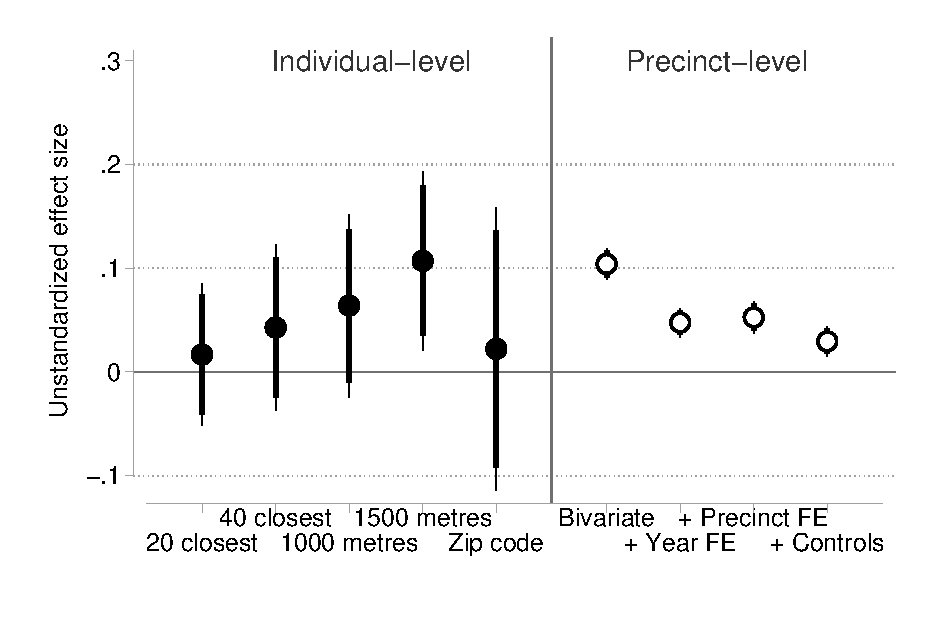
\includegraphics[width=0.9\textwidth]{../figures/comparison.eps}
		\centering
		\caption{Effects of Housing Prices across levels of analysis with 90  and 95 pct. Confidence Intervals}\label{comparison}
	\end{figure}
	
	As is clear from the figure, the effect sizes are similar across the two levels of analysis. If anything, the estimated effects appear slightly larger for the individual-level data. This tentatively suggests that that the estimated coefficients do not represent a true null-effect, but rather an imprecisely estimated effect. One plausible reason for this imprecision is measurement error in the dependent variable as voter recall data are known to be erroneously reported. In sum, we find mixed support for \hone in the individual level data, as the effect of housing prices is statistically insignificant in most specifications but comparable in sign and magnitude to the precinct-level results.
	
	We now test \htwo using the individual level data. Following our contextual priming-argument, we expect those who recently interacted with their local housing market to have considerations regarding the market more readily available when evaluating the incumbent government. One such group is those who have just moved or who are on the cusp of moving, as they are currently, or have recently, been exposed to information regarding local housing markets as a result of looking for a new home. 
	
	Table \ref{tabmovers} show that this group of movers are in fact significantly more responsive to changes in local housing prices. In particular, the table presents a set of re-estimated individual-level models from table \ref{inddv}, where the the housing price change variable is interacted with an indicator for whether or not the respondent is a mover (i.e., those who moved six months before/after being surveyed). The estimated interaction effect is statistically significant and positive in all specifications ($p<.05$ for all models except the zip-code model,$p<.1$ for the zip-code model). The results thus support the notion that  changes in local housing prices play a larger role in incumbent evaluations among individuals interacting with the local housing market.
	
	Figure \ref{move} presents marginal effects for movers and non-movers derived from these models. As shown, housing prices have a large estimated effect for movers and negligible effects for non-movers.  Only among movers is the effect of housing prices is significantly different from zero ($p<.05$ for all models except the zip-code model, $p<.1$ for the zip-code model.
	
	\begin{table}[htbp]\centering
\def\sym#1{\ifmmode^{#1}\else\(^{#1}\)\fi}
\caption{Linear Regression of Voting for Governing party } \footnotesize \label{tabmovers}
\begin{tabular}{l*{5}{c}}
\hline\hline
                    &\multicolumn{1}{c}{20 Closest}&\multicolumn{1}{c}{40 Closest}&\multicolumn{1}{c}{1000 metres}&\multicolumn{1}{c}{1500 metres}&\multicolumn{1}{c}{Zip code}\\
\hline
$\Delta$ housing prices&      -0.005       &       0.021       &       0.040       &       0.086\sym{+}&      -0.010       \\
                    &     (0.038)       &     (0.044)       &     (0.046)       &     (0.046)       &     (0.073)       \\
[1em]
Mover               &       0.010       &       0.012       &       0.004       &       0.025       &       0.030       \\
                    &     (0.030)       &     (0.031)       &     (0.036)       &     (0.032)       &     (0.031)       \\
[1em]
$\Delta$ housing prices $\times$ Mover&       0.180\sym{*}&       0.233\sym{*}&       0.266\sym{*}&       0.304\sym{*}&       0.377\sym{*}\\
                    &     (0.084)       &     (0.108)       &     (0.121)       &     (0.111)       &     (0.148)       \\
[1em]
Unemployment rate (context)&       0.260       &       0.259       &      -0.491       &       0.740       &       0.772\sym{+}\\
                    &     (0.374)       &     (0.375)       &     (0.634)       &     (0.586)       &     (0.421)       \\
[1em]
Average income (context)&      -0.002       &      -0.002       &      -0.005       &      -0.004       &      -0.005       \\
                    &     (0.004)       &     (0.004)       &     (0.007)       &     (0.007)       &     (0.006)       \\
[1em]
Personal income     &      -0.000       &      -0.000       &      -0.000       &      -0.000       &      -0.000       \\
                    &     (0.000)       &     (0.000)       &     (0.001)       &     (0.001)       &     (0.000)       \\
[1em]
Unnemployed (household)&      -0.034       &      -0.034       &      -0.070       &      -0.054       &      -0.033       \\
                    &     (0.035)       &     (0.035)       &     (0.043)       &     (0.040)       &     (0.036)       \\
[1em]
\hline  Round FE    &         Yes       &         Yes       &         Yes       &         Yes       &         Yes       \\
[1em]
Voter FE            &         Yes       &         Yes       &         Yes       &         Yes       &         Yes       \\
\hline
Observations        &        3479       &        3479       &        2790       &        2992       &        3392       \\
\hline\hline
\multicolumn{6}{l}{\footnotesize Standard errors in parentheses}\\
\multicolumn{6}{l}{\footnotesize \sym{+} \(p<0.1\), \sym{*} \(p<0.05\)}\\
\end{tabular}
\end{table}

	
	\begin{figure}[htbp!]
		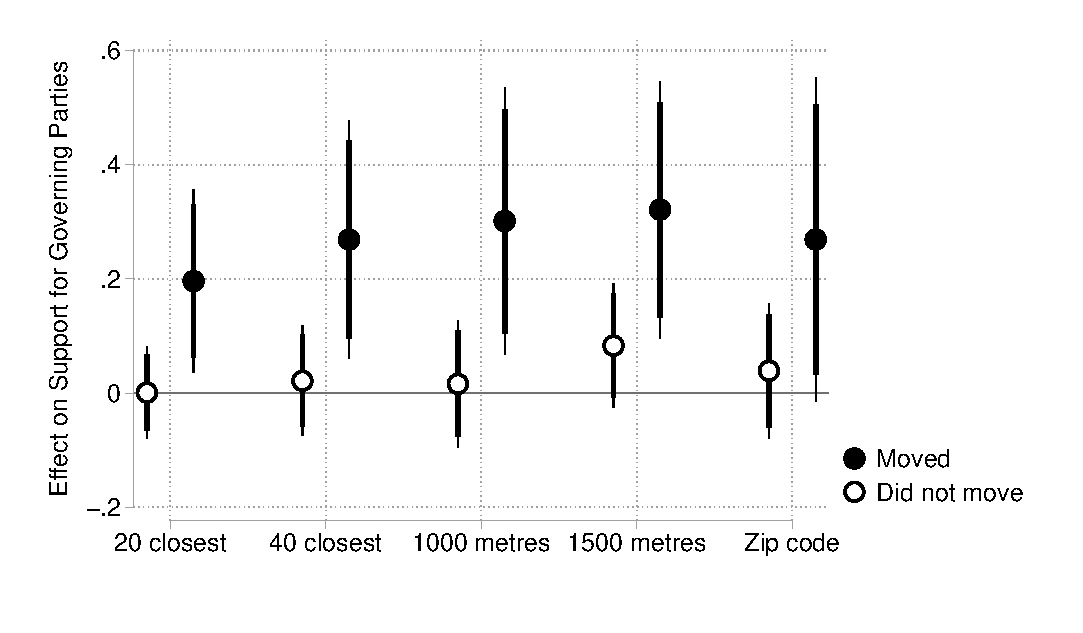
\includegraphics[width=0.9\textwidth]{../figures/moving.eps}
		\centering
		\caption{Effects of Changes in Housing Prices for those who had just or were going to move and those who did not with 90 and 95 pct. Confidence Intervals}\label{move}
	\end{figure}
	
	
	\subsection{Auxiliary analyses and robustness checks}
	
	Although the data is more constrained in terms of number of observations and number of time periods, we also conducted a number of supplementary analyses of the individual-level data (see Appendix \ref{app_robustind} for detailed results of these additional analyses). For one, we tried to re-estimate the models using a conditional logit model (i.e. logit with unit fixed effects). This takes into account that the dependent variable is dichotomous. However, it also entails all observations which do not change voting behavior between the two periods. These logit models reveal the same basic pattern as the linear models. The only important difference is that the zip-code interaction coefficient becomes statistically significant at the five percent level as well. 
	
	As an additional check, we examined whether the effect of local housing prices varies by home ownership status. In most models we find a positive, yet statistically insignificant interaction. Finally, following the party-specific analysis for the precinct-level data, which explored whether voters’ responses to local economic conditions had an ideological bent, we look at whether changes in local housing prices affect voters self-placement on a ten point left to right ideological scale. The estimated effects are generally small, statistically insignificant, and negative, suggesting that if anything, voters become more left-wing as housing prices increase.
	
	All in all, these analyses suggest that voter’s decision to support the sitting government is partly based on changes in local housing prices, and even more so for those particularly attuned to the housing market.
	
	\section{Conclusion}
	Trends in local housing prices tells you something fundamental about the state of the economy in a community. Just like unemployment or local economic growth, housing prices shape the experience and the fate of a community. For that reason, housing prices are likely to play an important role in politics (citep/Ansell2014). In this article we examined one possible political effect of changes in local housing prices: support for incumbents parties. Using precinct-level data on four Danish Parliamentary elections bookended by a dramatic bubble in real-estate prices, we found a positive effect of changes in housing prices on electoral support. Our results suggest that as housing prices increase, so does electoral support for governing parties. The effect is stronger in areas with more active markets, where housing prices are likely to be more salient to voters. Linking a two-wave panel survey of Danish voters to the national Danish registers, we replicated this finding, identifying a comparable effect of housing prices on incumbent support. Analyzing the panel data in more detail, we found that the effect of housing prices is especially pronounced among those who were more likely to be attuned to the local housing market. 
	
	
	Sig noget om implikationer af vores teori og hvordan den bør undersøges i fremtidige studier.
	
	What are the implications of our findings? First, politicians should care about housing prices and the policies that influence them. If they don’t, they risk facing electoral retribution. Further, since voters are sensitive to  local differences in housing prices, politicians cannot simply be attentive to national housing prices, but have to worry about the geographic distribution of any housing booms and busts \citep[cf.][11]{ferejohn1986incumbent}. Finding that voters care about local economic conditions, is especially interesting in light of the fact that most studies of the electoral effects of the economy have focused on the national economy or, to a lesser extent, personal economic conditions.
	
	Add discussion of irrationality in light of this. Perhaps, that this is consistent with a macro level rationality in that people will learn something about the parts of the economy that they interact with, and that this will often be important parts of the economy, leading to a relationship between the importance of a type of local economic conditions and whether incumbents will be held accountable.
	
	The data used in this study are an improvement over those used in earlier studies; we have applied highly stringent tests of our hypotheses and rigorously probed the robustness of our results including assessing potential confounding. Yet, our data are nonetheless observational and in the absence of fully or quasi-experimental variation in housing prices, we cannot be sure that the estimated effects are not confounded by unobserved heterogeneity. Building on this study, a promising avenue for future research is to identify settings with plausibly exogenous variation \citep[cf.]{jerzak2016property}.
	
	
	
	
	
	
	
	
	
	
	
	\clearpage
	
	\singlespacing
	
	\bibliographystyle{apa}
	\bibliography{library}
	
	\newpage
	
	\appendix
	\section*{Appendix}
		\onehalfspacing
	\renewcommand{\thesubsection}{\Alph{subsection}}
	\renewcommand{\thetable}{\Alph{subsection}\arabic{table}}
	\renewcommand{\thefigure}{\Alph{subsection}\arabic{figure}}
	
	\localtableofcontents

	
	\newpage
	
	\subsection{Linking polling places to zip codes}\label{app_linking}
	
	Zip codes are a substantively interesting level of aggregation when it comes to the price of housing, as it is the level at which housing prices are most often reported in Denmark (cf. the fact they are published by The Danish Mortgage Banks' Federation). However, merging zip code-level data on housing prices to the precinct-level data on electoral outcomes is non-trivial. Ideally we would extract the zip code of the address of each polling place and link the polling place to housing prices in that zip code. Unfortunately, full addresses are not available for all polling places. Instead, we use a three-stage approach to linking polling places to zip codes. First, we extract the street address and higher-level voting district of each polling place (the full resulting string is of the format `Streetname streetnumber, City, Denmark'). Second, we pass this string to the Google Maps API, which geocodes the string and returns latitude-longitude coordinates.\footnote{Available at \texttt{\href{https://developers.google.com/maps/documentation/geocoding/intro}{developers.google.com/maps/documentation/geocoding/intro}}.} Third and last, we pass these coordinates to the Danish Addresses Web API (DAWA), a public service provided by the Danish Geodata Agency.\footnote{Available at \texttt{\href{http://dawa.aws.dk/}{dawa.aws.dk}}.} The DAWA returns the zip code for each address, allowing us to link polling places to zip codes. %It is important to note that statistically speaking, precincts are therefore nested inside zip codes; we take this into account by clustering the standard errors on the precinct-level in our analysis.
	
	\newpage
	
	\subsection{Estimates of  Local Housing Prices}\label{app_housingselect}
	
	We use all housing sales registered in the national register EJSA except for those that fall into one or more of the following categories:
	
	\begin{enumerate}
		\item Sales of part of a house or apartment (10 pct. of all sales). We exclude these as these are typically quasi-commercial, as part of a house or apartment is sold to a business. Many of these sales are between farmers who sell and buy land from one another.
		\item Sales of commercial real estate (9 pct). These are excluded because we are interested in residential real-estate.
		\item Sales of apartments or houses valued at more than DKK 10 million (0.2 pct. of all sales). These are considered outliers, which tell us little about the state of the local housing market experienced by the typical Danish voter.
		\item Sales with what Statistics Denmark calls an irregular price (i.e. if the sales price is more than three times the valuation or less than forty percent of the valuation, 6 pct. of all sales). This will usually mean that sellers and buyers are not part of the regular housing market (e.g., family members or friends selling or buying).
	\end{enumerate}
	
	For more details on the EJSA register see \texttt{\href{http://www.dst.dk/extranet/ForskningVariabellister/EJSA\%20-\%20Ejendomme\%20salgsoplysninger.html}{http://www.dst.dk/}}.

	\newpage		
			\subsection{Descriptive statistics}
			\setcounter{table}{0}
			
			Descriptive statistics for the precinct-level data can be found in table \ref{desall}. Descriptive statistics for the individual-level data can be found in table \ref{sumstat}. We do not include maximum and minimum values for the individual level variables, because this would go against the guidelines provided by Statstics Denmark.
			
			\input{../tables/predes.txt}
			
\begin{table}[htbp]\centering \caption{Descriptive Statistics, Individual-level data \label{sumstat}}
\begin{tabular}{l c c  c}\hline\hline
\multicolumn{1}{c}{\textbf{Variable}} & \textbf{Mean}
 & \textbf{Std. Dev.} & \textbf{N}\\ \hline
Left/Right Scale & 0.532 & 0.217  & 3350\\
Unnemployed (household) & 0.062 & 0.241  & 3483\\
Unemployment rate 1000 meters & 0.067 & 0.035  & 3481\\
Unemployment rate 1500 meters & 0.068 & 0.031  & 3481\\
Home Owner & 0.736 & 0.441  & 3451\\
$\Delta$ housing price 1000 meters & -0.05 & 0.236  & 2792\\
Avberage income 1000 meters & 17.915 & 3.905  & 3481\\
$\Delta$ housing price 1500 meters & -0.051 & 0.227  & 2994\\
Average income 1500 meters & 17.892 & 3.624  & 3481\\
Personal income & 20.859 & 22.277  & 3486\\
$\Delta$ housing price zip code & -0.066 & 0.138  & 3396\\
$\Delta$ housing price 20 closest & -0.046 & 0.218  & 3482\\
$\Delta$ housing price 40 closest & -0.05 & 0.182  & 3482\\
Vote for Government Party & 0.299 & 0.458  & 3486\\
Mover & 0.077 & 0.267  & 3486\\
\hline\end{tabular}
\end{table}

			
			
			\newpage
			
			\subsection{Identification strategy}
			
			In this article we want to identify the causal effect of recent changes in precinct level housing prices on electoral support for governing parties. Ideally, we would like to compare support for governing parties in the same district at a specific election across different levels of house-prices. As precincts were only assigned one change in housing prices per election, this is obviously not feasible. Instead, we need to construct a feasible observable counterfactual to a precinct with a specific change in housing prices, which we can use to difference out the effect of housing prices.
			
			One way to do this is to simply compare incumbent support at different levels of housing price changes across elections and within precincts. Here the counterfactual for any given precinct is the incumbent support of an cross-elections average precinct. A key challenge to causal identification in this case is that certain structural features of precincts in which housing prices are likely to increase might make incumbents more popular.
			
			We can begin to deal with this problem by examining the historical precinct-specific levels of incumbent support. As such, instead of simply using an average of all precincts as our counterfactual, we can use the average for the individual precinct. Comparing incumbent support within precincts and across different levels of housing prices. This takes into account that certain precincts might be historically more inclined to support incumbents and have increasing housing prices. However, it does not take into account that when housing prices are relatively high in a district in a particular election, it is also likely to be high in other precincts as well. This is problematic if incumbents do systematically better or worse, in general, when housing prices are doing well.
			
			To address this problem, we can examine levels of incumbents support, not just relative to the precincts history, but also relative to the level of incumbent support across districts. In this case, our counterfactual for any given precinct is the electoral support that governing parties typically obtain in that precinct, plus or minus the overall change in electoral support for governing parties across all precincts. This is a generalized difference-in-difference approach to identifying the effect of housing prices. As such, we look at differences within elections in differences between the individual precincts typical and actual outcome.
			
			The difference-in-differences approach makes it possible to compare with a very reasonable counterfactual situation -- what is the typical incumbent support we could expect in a precinct given the overall popularity of the incumbent. However, since the the governing parties change from election to election, and since the priorities of the same parties might change from election to election, different types of precincts might prefer government parties at  different elections. This poses a challenge to causal identification. As such,  these changes in election and precinct-specific preferences might not be the same across types of precincts which experience increasing and decreasing in housing prices. We cannot completely deal with this problem: As mentioned in the beginning of this section, we have only one piece of information on the assigned housing price change for a precinct at an individual election. However, we can create an even more appropriate counter-factual by taking into account how precincts of a specific type do at specific elections. In particular, we hold constant the economic conditions in the precinct by controlling for precinct-level unemployment rate and median income.
			
			\newpage
			
			\subsection{Party Specific analysis in precinct-level data} \label{app_partyspec}
			\setcounter{table}{0}
			
			Table \ref{partyspecifictab} presents the estimates for the model underlying Figure \ref{partyspecific}. 
			

			
			\begin{table}[htbp]\centering
\def\sym#1{\ifmmode^{#1}\else\(^{#1}\)\fi}
\caption{Party Specific Analysis.} \label{partyspecifictab}
\begin{tabular}{l*{1}{c}}
\hline\hline
                    &\multicolumn{1}{c}{(1)}        \\
\hline
$\Delta$ housing price&       0.083\sym{**}\\
                    &     (0.007)        \\
[1em]
$\Delta$ housing price $\times$ Left-wing Incumbent&      -0.123\sym{**}\\
                    &     (0.016)        \\
[1em]
$\Delta$ housing price $\times$ Left-wing Support&      -0.146\sym{**}\\
                    &     (0.010)        \\
[1em]
Left-wing Incumbent $\times$ Left-wing Support&      10.651\sym{**}\\
                    &     (0.233)        \\
[1em]
$\Delta$ housing price $\times$ Left-wing Incumbent $\times$ Left-wing Support&       0.284\sym{**}\\
                    &     (0.025)        \\
[1em]
Unemployment rate   &       0.104        \\
                    &     (0.080)        \\
[1em]
Median income (1000 DKK)&      -0.002        \\
                    &     (0.021)        \\
[1em]
\hline Precinct FE  &$\checkmark$        \\
[1em]
Year FE             &$\checkmark$        \\
\hline
Observations        &        8358        \\
RMSE                &       7.727        \\
\hline\hline
\multicolumn{2}{l}{\footnotesize Standard errors in parentheses}\\
\multicolumn{2}{l}{\footnotesize \sym{*} \(p<0.05\), \sym{**} \(p<0.01\)}\\
\end{tabular}
\end{table}

			
			\newpage
			
			\subsection{Full Models from Robustness Checks of Precinct-level Evidence} \label{app_robustpred}
			\setcounter{table}{0}
			
			Table \ref{apdxprerobust} presents the models shown in table \ref{robustness} with covariates.
			
			\begin{sidewaystable}[htbp]\centering
\def\sym#1{\ifmmode^{#1}\else\(^{#1}\)\fi}
\caption{Robustness checks of the Precinct-level data.} \label{apdxprerobust}
\begin{tabular}{l*{12}{c}}
\hline\hline
                    &\multicolumn{1}{c}{(1)}        &\multicolumn{1}{c}{(2)}        &\multicolumn{1}{c}{(3)}        &\multicolumn{1}{c}{(4)}        &\multicolumn{1}{c}{(5)}        &\multicolumn{1}{c}{(6)}        &\multicolumn{1}{c}{(7)}        &\multicolumn{1}{c}{(8)}        &\multicolumn{1}{c}{(9)}        &\multicolumn{1}{c}{(10)}        &\multicolumn{1}{c}{(11)}        &\multicolumn{1}{c}{(12)}        \\
\hline
$\Delta$ housing price&       0.030\sym{**}&      -0.079\sym{**}&                    &                    &       0.058\sym{**}&      -0.105\sym{**}&       0.027\sym{**}&       0.010        &       0.060\sym{**}&      -0.207\sym{**}&                    &                    \\
                    &     (0.007)        &     (0.023)        &                    &                    &     (0.008)        &     (0.024)        &     (0.005)        &     (0.016)        &     (0.008)        &     (0.029)        &                    &                    \\
$\Delta$ housing price (2 years)&                    &                    &       0.020\sym{**}&      -0.042\sym{**}&                    &                    &                    &                    &                    &                    &                    &                    \\
                    &                    &                    &     (0.007)        &     (0.015)        &                    &                    &                    &                    &                    &                    &                    &                    \\
$\Delta$ housing price (positive)&                    &                    &                    &                    &                    &                    &                    &                    &                    &                    &       0.030\sym{**}&      -0.229\sym{**}\\
                    &                    &                    &                    &                    &                    &                    &                    &                    &                    &                    &     (0.011)        &     (0.040)        \\
$\Delta$ housing price (negative)&                    &                    &                    &                    &                    &                    &                    &                    &                    &                    &      -0.029        &      -0.168\sym{**}\\
                    &                    &                    &                    &                    &                    &                    &                    &                    &                    &                    &     (0.019)        &     (0.060)        \\
Log(trades)         &                    &       1.995\sym{**}&                    &       2.002\sym{**}&                    &       3.480\sym{**}&                    &       0.671\sym{**}&                    &       0.225\sym{**}&                    &       1.268\sym{*} \\
                    &                    &     (0.484)        &                    &     (0.474)        &                    &     (0.525)        &                    &     (0.237)        &                    &     (0.080)        &                    &     (0.545)        \\
$\Delta$ housing price $\times$ Log(trades)&                    &       0.033\sym{**}&                    &                    &                    &       0.048\sym{**}&                    &       0.005        &                    &       0.089\sym{**}&                    &                    \\
                    &                    &     (0.007)        &                    &                    &                    &     (0.008)        &                    &     (0.005)        &                    &     (0.010)        &                    &                    \\
$\Delta$ housing price (2 years) $\times$ Log(trades)&                    &                    &                    &       0.017\sym{**}&                    &                    &                    &                    &                    &                    &                    &                    \\
                    &                    &                    &                    &     (0.005)        &                    &                    &                    &                    &                    &                    &                    &                    \\
$\Delta$ housing price (positive) $\times$ Log(trades)&                    &                    &                    &                    &                    &                    &                    &                    &                    &                    &                    &       0.080\sym{**}\\
                    &                    &                    &                    &                    &                    &                    &                    &                    &                    &                    &                    &     (0.013)        \\
$\Delta$ housing price (negative) $\times$ Log(trades)&                    &                    &                    &                    &                    &                    &                    &                    &                    &                    &                    &       0.049\sym{*} \\
                    &                    &                    &                    &                    &                    &                    &                    &                    &                    &                    &                    &     (0.019)        \\
Log(Median income)  &      -0.887\sym{**}&      -0.855\sym{**}&      -0.935\sym{**}&      -0.909\sym{**}&                    &                    &       0.150\sym{**}&       0.170\sym{**}&      -0.034\sym{**}&      -0.025\sym{**}&      -0.887\sym{**}&      -0.869\sym{**}\\
                    &     (0.064)        &     (0.063)        &     (0.060)        &     (0.060)        &                    &                    &     (0.019)        &     (0.019)        &     (0.008)        &     (0.008)        &     (0.064)        &     (0.064)        \\
Unemployment rate   &      -1.904\sym{**}&      -1.649\sym{**}&      -1.952\sym{**}&      -1.662\sym{**}&                    &                    &       0.098        &       0.221\sym{*} &      -0.220\sym{**}&      -0.202\sym{**}&      -1.904\sym{**}&      -1.726\sym{**}\\
                    &     (0.221)        &     (0.217)        &     (0.225)        &     (0.223)        &                    &                    &     (0.101)        &     (0.112)        &     (0.040)        &     (0.041)        &     (0.222)        &     (0.222)        \\
Log(Median income) (change)&                    &                    &                    &                    &      -0.000\sym{**}&      -0.000\sym{**}&                    &                    &                    &                    &                    &                    \\
                    &                    &                    &                    &                    &     (0.000)        &     (0.000)        &                    &                    &                    &                    &                    &                    \\
Unemployment rate (change)&                    &                    &                    &                    &       0.005        &       0.003        &                    &                    &                    &                    &                    &                    \\
                    &                    &                    &                    &                    &     (0.215)        &     (0.216)        &                    &                    &                    &                    &                    &                    \\
L.Support for Governing Parties (pct.)&                    &                    &                    &                    &                    &                    &                    &                    &       0.513\sym{**}&       0.515\sym{**}&                    &                    \\
                    &                    &                    &                    &                    &                    &                    &                    &                    &     (0.008)        &     (0.008)        &                    &                    \\
\hline Precinct FE  &$\checkmark$        &$\checkmark$        &$\checkmark$        &$\checkmark$        &$\checkmark$        &$\checkmark$        &$\checkmark$        &$\checkmark$        &                    &                    &$\checkmark$        &$\checkmark$        \\
Year FE             &$\checkmark$        &$\checkmark$        &$\checkmark$        &$\checkmark$        &$\checkmark$        &$\checkmark$        &$\checkmark$        &$\checkmark$        &$\checkmark$        &$\checkmark$        &$\checkmark$        &$\checkmark$        \\
\hline
Observations        &        4179        &        4179        &        4163        &        4163        &        4179        &        4179        &        3091        &        3091        &        3091        &        3091        &        4179        &        4179        \\
RMSE                &       5.325        &       5.288        &       5.246        &       5.218        &       5.690        &       5.592        &       2.124        &       2.119        &       6.252        &       6.153        &       5.326        &       5.278        \\
\hline\hline
\multicolumn{13}{l}{\footnotesize Standard errors in parentheses}\\
\multicolumn{13}{l}{\footnotesize Models 7 and 8 have a first-differenced version of the dependent variable.}\\
\multicolumn{13}{l}{\footnotesize \sym{*} \(p<0.05\), \sym{**} \(p<0.01\)}\\
\end{tabular}
\end{sidewaystable}
 
			
			\newpage
			
			\subsection{Full Models from Robustness Checks of Individual-level Evidence} \label{app_robustind}
			
			\setcounter{table}{0}
			
			Tables \ref{logit} and \ref{logitinter} re-estimates the linear regression models presented in table \ref{inddv} and \ref{tabmovers} using conditional logit models.
			
			Table  \ref{home} present the results of the home-ownership by housing price interaction.
			
			Table \ref{lrscale} examines the relationship between changes in housing prices and  self-placement on an ideological left-right scale.
			
			\begin{table}[htbp]\centering
\def\sym#1{\ifmmode^{#1}\else\(^{#1}\)\fi}
\caption{Linear Regression of Voting for Governing party } \footnotesize \label{logit}
\begin{tabular}{l*{5}{c}}
\hline\hline
                    &\multicolumn{1}{c}{20 Closest}&\multicolumn{1}{c}{40 Closest}&\multicolumn{1}{c}{1000 metres}&\multicolumn{1}{c}{1500 metres}&\multicolumn{1}{c}{Zip code}\\
\hline
%incumbent support  &                   &                   &                   &                   &                   \\
$\Delta$ housing prices&       0.331       &       0.657       &       0.846\sym{+}&       1.217\sym{*}&       0.097       \\
                    &     (0.492)       &     (0.633)       &     (0.467)       &     (0.545)       &     (0.753)       \\
[1em]
Unemployment rate (context)&       3.177       &       3.053       &      -4.854       &      12.371\sym{+}&      12.557\sym{+}\\
                    &     (5.122)       &     (5.120)       &     (6.602)       &     (7.419)       &     (6.781)       \\
[1em]
Average income (context)&      -0.045       &      -0.046       &      -0.073       &      -0.078       &      -0.058       \\
                    &     (0.048)       &     (0.048)       &     (0.061)       &     (0.073)       &     (0.058)       \\
[1em]
Personal income     &      -0.001       &      -0.001       &       0.000       &      -0.000       &      -0.002       \\
                    &     (0.003)       &     (0.003)       &     (0.003)       &     (0.003)       &     (0.004)       \\
[1em]
Unnemployed (household)&      -0.203       &      -0.191       &      -0.524       &      -0.245       &      -0.234       \\
                    &     (0.476)       &     (0.477)       &     (0.614)       &     (0.584)       &     (0.487)       \\
[1em]
\hline  Round FE    &         Yes       &         Yes       &         Yes       &         Yes       &         Yes       \\
[1em]
Voter FE            &         Yes       &         Yes       &         Yes       &         Yes       &         Yes       \\
\hline
Observations        &         622       &         622       &         458       &         496       &         608       \\
\hline\hline
\multicolumn{6}{l}{\footnotesize Standard errors in parentheses}\\
\multicolumn{6}{l}{\footnotesize \sym{+} \(p<0.1\), \sym{*} \(p<0.05\)}\\
\end{tabular}
\end{table}

			\begin{table}[htbp]\centering
\def\sym#1{\ifmmode^{#1}\else\(^{#1}\)\fi}
\caption{Conditional Logit Regression of Voting for Governing party} \label{logitinter}
\begin{tabular}{l*{5}{c}}
\hline\hline
                    &\multicolumn{1}{c}{20 Closest}&\multicolumn{1}{c}{40 Closest}&\multicolumn{1}{c}{1000 metres}&\multicolumn{1}{c}{1500 metres}&\multicolumn{1}{c}{Zip code}\\
\hline
%incumbent support  &                   &                   &                   &                   &                   \\
$\Delta$ housing prices&       0.039       &       0.465       &       0.479       &       0.915\sym{+}&      -0.186       \\
                    &     (0.512)       &     (0.643)       &     (0.491)       &     (0.540)       &     (0.767)       \\
[1em]
Mover               &       0.079       &       0.037       &      -0.026       &       0.716       &       0.844\sym{+}\\
                    &     (0.367)       &     (0.363)       &     (0.421)       &     (0.482)       &     (0.506)       \\
[1em]
$\Delta$ housing prices $\times$ Mover&       4.052\sym{*}&       5.303\sym{*}&       4.565\sym{*}&       7.713\sym{*}&      10.299\sym{*}\\
                    &     (1.884)       &     (2.421)       &     (2.063)       &     (2.910)       &     (3.838)       \\
[1em]
Unemployment rate (context)&       1.870       &       3.174       &      -6.715       &      13.059\sym{+}&      14.467\sym{*}\\
                    &     (5.237)       &     (5.236)       &     (6.781)       &     (7.672)       &     (6.861)       \\
[1em]
Average income (context)&      -0.040       &      -0.042       &      -0.073       &      -0.082       &      -0.048       \\
                    &     (0.048)       &     (0.048)       &     (0.063)       &     (0.076)       &     (0.058)       \\
[1em]
Personal income     &      -0.001       &      -0.001       &       0.000       &      -0.000       &      -0.002       \\
                    &     (0.003)       &     (0.003)       &     (0.003)       &     (0.003)       &     (0.004)       \\
[1em]
Unnemployed (household)&      -0.226       &      -0.201       &      -0.526       &      -0.191       &      -0.194       \\
                    &     (0.478)       &     (0.480)       &     (0.624)       &     (0.598)       &     (0.496)       \\
[1em]
\hline  Round FE    &         Yes       &         Yes       &         Yes       &         Yes       &         Yes       \\
[1em]
Voter FE            &         Yes       &         Yes       &         Yes       &         Yes       &         Yes       \\
\hline
Observations        &         622       &         622       &         458       &         496       &         608       \\
\hline\hline
\multicolumn{6}{l}{\footnotesize Standard errors in parentheses}\\
\multicolumn{6}{l}{\footnotesize \sym{+} \(p<0.1\), \sym{*} \(p<0.05\)}\\
\end{tabular}
\end{table}

			\begin{table}[htbp]\centering
\def\sym#1{\ifmmode^{#1}\else\(^{#1}\)\fi}
\caption{Linear Regression of Voting for Governing party } \footnotesize \label{home}
\begin{tabular}{l*{5}{c}}
\hline\hline
                    &\multicolumn{1}{c}{20 Closest}&\multicolumn{1}{c}{40 Closest}&\multicolumn{1}{c}{1000 metres}&\multicolumn{1}{c}{1500 metres}&\multicolumn{1}{c}{Zip code}\\
\hline
$\Delta$ housing price&       0.043       &       0.030       &       0.043       &       0.029       &      -0.101       \\
                    &     (0.047)       &     (0.056)       &     (0.068)       &     (0.081)       &     (0.096)       \\
[1em]
Home Owner          &      -0.014       &      -0.012       &      -0.025       &      -0.016       &      -0.012       \\
                    &     (0.033)       &     (0.033)       &     (0.041)       &     (0.038)       &     (0.035)       \\
[1em]
$\Delta$ housing price $\times$ Home Owner&      -0.047       &       0.024       &       0.001       &       0.096       &       0.171       \\
                    &     (0.060)       &     (0.072)       &     (0.079)       &     (0.088)       &     (0.105)       \\
[1em]
Unemployment rate (context)&       0.147       &       0.134       &      -0.786       &       0.500       &       0.296       \\
                    &     (0.393)       &     (0.391)       &     (0.651)       &     (0.596)       &     (0.627)       \\
[1em]
Average income (context)&      -0.003       &      -0.003       &      -0.007       &      -0.006       &      -0.013\sym{+}\\
                    &     (0.004)       &     (0.004)       &     (0.007)       &     (0.007)       &     (0.007)       \\
[1em]
Personal income     &      -0.000       &      -0.000       &      -0.000       &      -0.000       &      -0.000       \\
                    &     (0.000)       &     (0.000)       &     (0.001)       &     (0.001)       &     (0.000)       \\
[1em]
Unnemployed (household)&      -0.024       &      -0.024       &      -0.060       &      -0.043       &      -0.022       \\
                    &     (0.036)       &     (0.036)       &     (0.044)       &     (0.042)       &     (0.037)       \\
[1em]
\hline  Round FE    &         Yes       &         Yes       &         Yes       &         Yes       &         Yes       \\
[1em]
Voter FE            &         Yes       &         Yes       &         Yes       &         Yes       &         Yes       \\
\hline
Observations        &        3447       &        3447       &        2767       &        2965       &        3372       \\
\hline\hline
\multicolumn{6}{l}{\footnotesize Standard errors in parentheses}\\
\multicolumn{6}{l}{\footnotesize \sym{+} \(p<0.1\), \sym{*} \(p<0.05\)}\\
\end{tabular}
\end{table}

			\begin{table}[htbp]\centering
\def\sym#1{\ifmmode^{#1}\else\(^{#1}\)\fi}
\caption{Linear Regression of Left-Right Self Placement (Ideology)} \footnotesize \label{lrscale}
\begin{tabular}{l*{5}{c}}
\hline\hline
                    &\multicolumn{1}{c}{20 Closest}&\multicolumn{1}{c}{40 Closest}&\multicolumn{1}{c}{1000 metres}&\multicolumn{1}{c}{1500 metres}&\multicolumn{1}{c}{Zip code}\\
\hline
$\Delta$ housing price&      -0.020       &      -0.016       &       0.018       &      -0.007       &      -0.002       \\
                    &     (0.022)       &     (0.021)       &     (0.024)       &     (0.019)       &     (0.031)       \\
[1em]
Unemployment rate (context)&      -0.298       &      -0.311       &      -0.392       &      -0.271       &      -0.297       \\
                    &     (0.242)       &     (0.238)       &     (0.300)       &     (0.281)       &     (0.297)       \\
[1em]
Average income (context)&      -0.001       &      -0.001       &       0.001       &       0.003       &       0.002       \\
                    &     (0.002)       &     (0.002)       &     (0.002)       &     (0.002)       &     (0.003)       \\
[1em]
Personal income     &       0.000       &       0.000       &       0.000\sym{*}&       0.000\sym{*}&       0.000       \\
                    &     (0.000)       &     (0.000)       &     (0.000)       &     (0.000)       &     (0.000)       \\
[1em]
Unnemployed (household)&      -0.021       &      -0.022       &      -0.039       &      -0.035       &      -0.021       \\
                    &     (0.020)       &     (0.020)       &     (0.025)       &     (0.023)       &     (0.021)       \\
[1em]
\hline  Round FE    &         Yes       &         Yes       &         Yes       &         Yes       &         Yes       \\
[1em]
Voter FE            &         Yes       &         Yes       &         Yes       &         Yes       &         Yes       \\
\hline
Observations        &        3343       &        3343       &        2683       &        2878       &        3262       \\
\hline\hline
\multicolumn{6}{l}{\footnotesize Standard errors in parentheses}\\
\multicolumn{6}{l}{\footnotesize \sym{+} \(p<0.1\), \sym{*} \(p<0.05\)}\\
\end{tabular}
\end{table}

			
			\newpage
			
			\subsection{The Interaction with Logged Number of Trades} \label{app_interaction}
			\setcounter{table}{0}
			\setcounter{figure}{0}
			
			Figure \ref{scatter} examines how strongly related logged number of trades is with changes in housing prices. As can be seen from this plot, there is a weak correlation between logged number of trades and changes in housing prices, but a stronger correlation between changes in logged number of trades and changes in housing prices. However, even though the correlation is stronger in the latter case, it is evident that there is a lot of independent variation in number of trades for different levels of housing prices, and, as such, it seems reasonable to use number of trades as a moderator.
			
			Figure \ref{terciles} uses the binning and kernel estimators developed by Hainmueller, Mummolo and Xu (2016) to test for linearity of the interaction. As can be seen from this model, the interaction does not seem to be perfectly linear. Rather, the marginal effect seems to low and stable at low and middling levels of number of trades, but then shoot up at high levels.
			
			\begin{figure}
				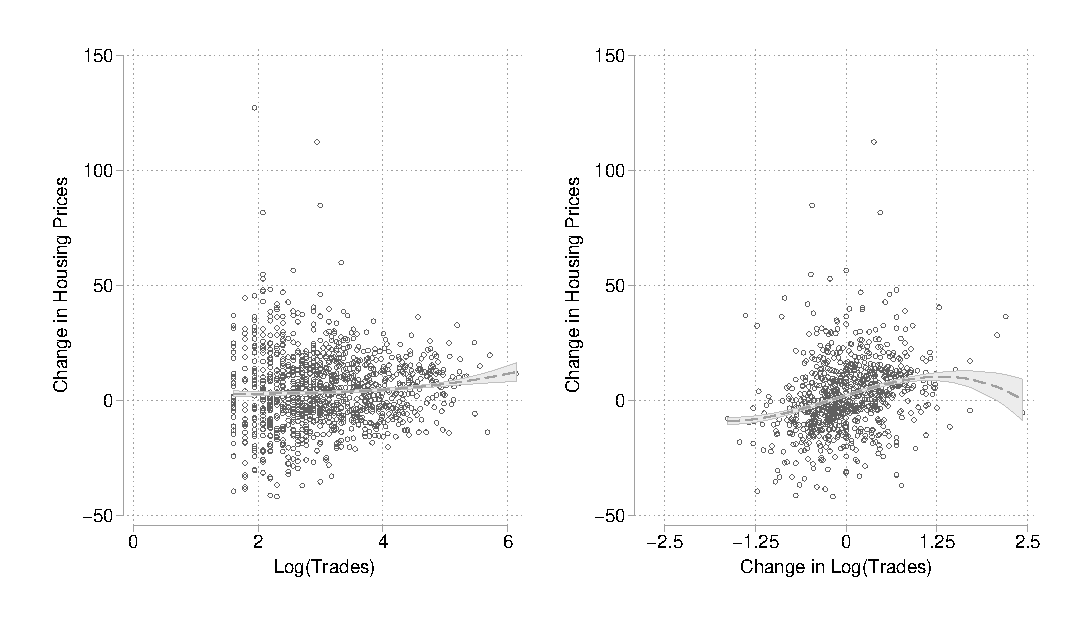
\includegraphics[width=1\textwidth]{../figures/corrmoderator.eps}
				\caption{How Closely Related is Number of Trades and Changes in Housing Prices? Dots are observations, line is fractional polynomial fit and area represents 95 pct. confidence interval of this fit. For number of trades the overall Pearson correlation with prices is $0.1$ ($n=3,100$), for the change variable it is $0.3$ ($n=4,199$). }
				\label{scatter}
			\end{figure}
			
			
			\begin{figure}
				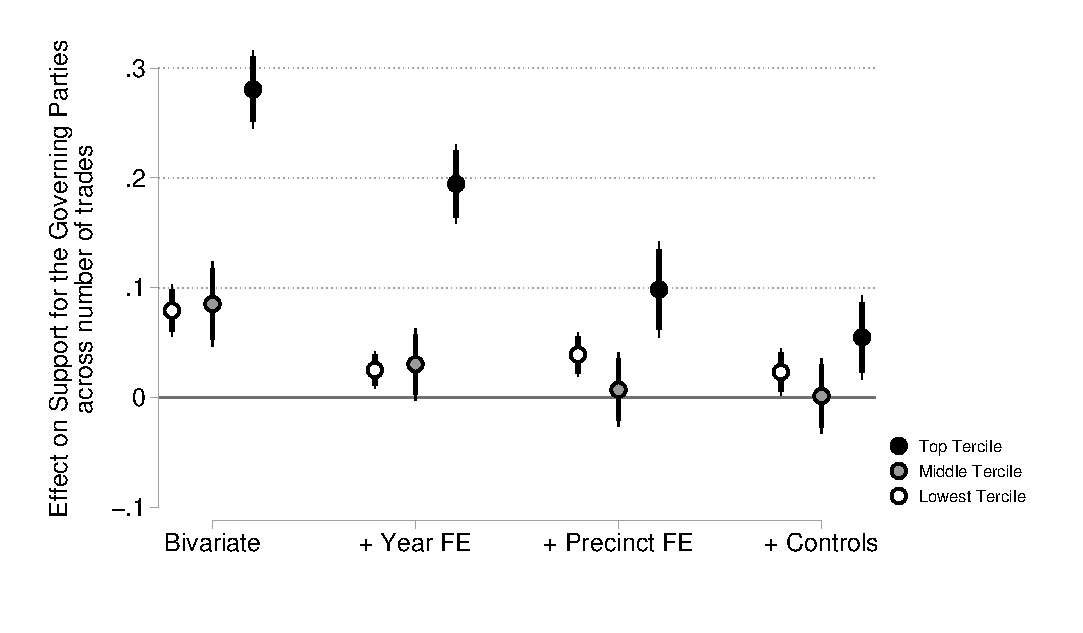
\includegraphics[width=0.7\textwidth]{../figures/localactivity_sup.eps}
				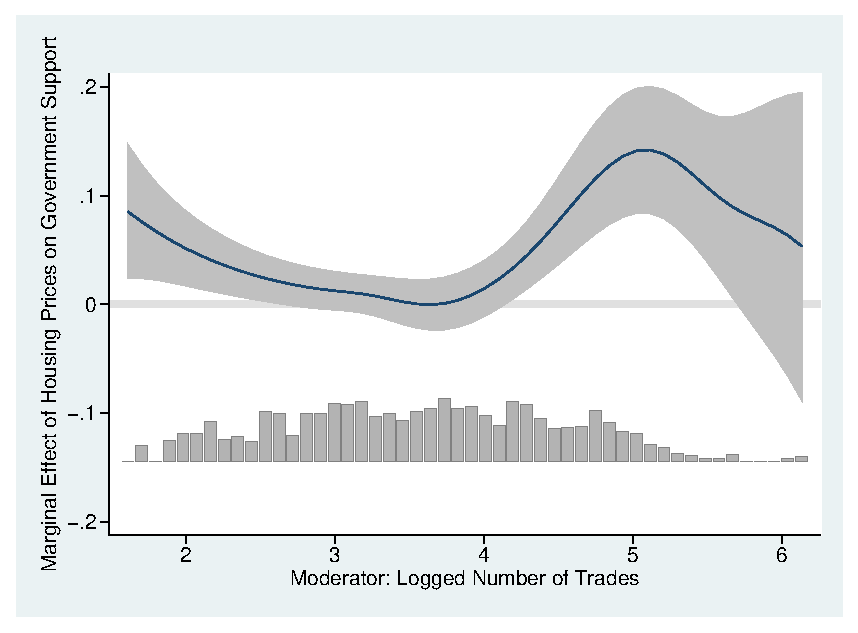
\includegraphics[width=0.7\textwidth]{../figures/localactivity_sup2.eps}
				
				\caption{Interaction estimation using the binning (top) and kernel estimators (bottom) developed by Hainmueller, Mummolo and Xu (2016). The binning estimator is applied to all four specification presented in table \ref{predv}. The kernel estimator is only applied to the most restrictive model including year and precint fixed effects as well as economic controls.}
				\label{terciles}
			\end{figure}
			
			
			
			
			
		\end{document}


